\section{Menü-Struktur}

% Siehe auch: https://sopra.informatik.uni-freiburg.de/soprawiki/Men%C3%BC

% Bei der Beschreibung der Menü-Struktur wird erklärt, wie das Hauptmenü und
% alle In-Game-Menüs zueinander in Beziehung stehen. Hilfreich dazu kann ein
% Diagramm in Form eines Graphen oder Baums sein.
%
% Wichtig ist, dass ersichtlich wird, welche Aktion im Menü welche Reaktion des
% Interfaces verursacht. Beispiel: "Wenn man im Einstellungsmenü auf 'Zurück'
% klickt, gelangt man zurück ins Hauptmenü."
%
% Ebenso wichtig ist die Vollständigkeit der Beschreibung. Jedes Menü und jedes
% Untermenü sollten erklärt werden.

% \missingSection{Menü-Struktur}

\begin{figure}[ht]
	\centering
	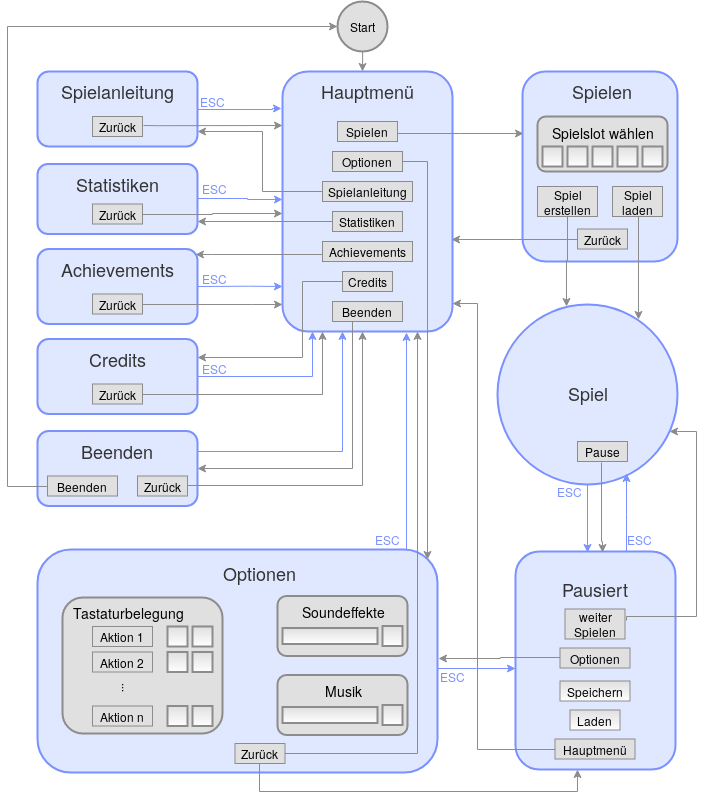
\includegraphics[width=1\textwidth]{menu_structure.png}
	\caption{Menü-Struktur}
	\label{menu}
\end{figure}


% 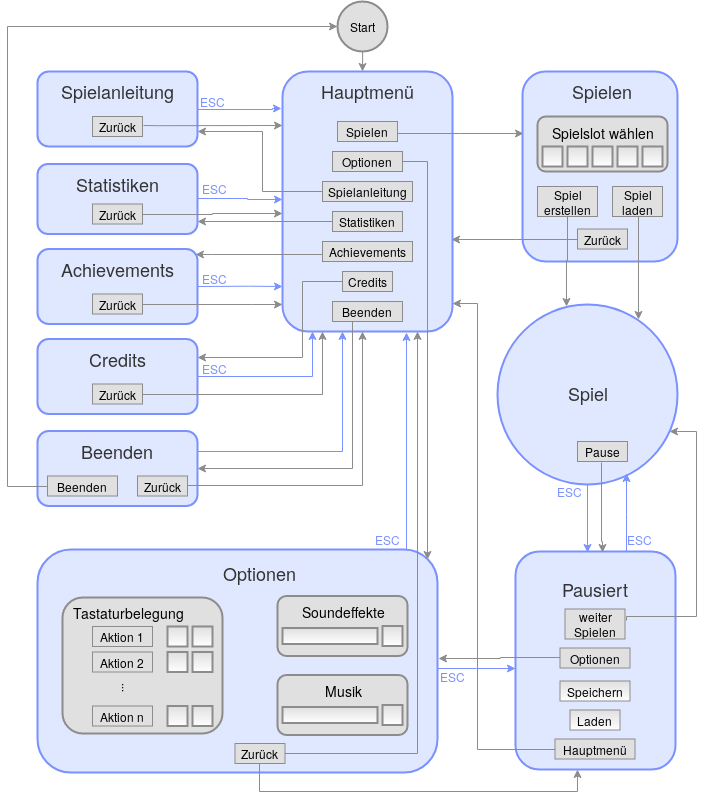
\includegraphics[width=\textwidth]{menu_structure.png}